\chapter{Especificação de Requisitos}
\label{sec:requisitos}



O processo de especificação de requisitos é crucial para o desenvilvimento de um projecto de \textit{software}, devendo dar atenção tanto aos requisitos funcionais como aos requisitos não funcionais.

Este capítulo apresenta os requisitos que foram identificados e analisados para a plataforma e define um conjunto de diretrizes que devem ser seguidas durante o desenvolvimento do projeto. Estes requisitios foram definidos e identificados com base em reuniões com o cliente e na analise de soluções, actualmente no mercado, que partilham funcionalidades semelhantes com a plataforma que vai ser desenvolvida

Este capítulo divide-se em 3 secções. A secção \ref{requisitos:tiposutilizadores} identifica as principais partes envolventes no projecto (i. e. utilizadores e utilizadores finais). A secção \ref{rnf} e \ref{rf} descreve, detalhadamente, os requisitos não funcionais e funcionais, respectivamente. Por fim temos a secção \ref{prototipagem} que apresenta uma prototipagem de baixo nível, que com auxílio de breves descrições representa o fluxo da plataforma.


\section{Tipos de Utilizadores}
\label{requisitos:tiposutilizadores}

O objectivo desta secção é identificar, não necessariamente um problema, mas sim, através de uma estratégia de inbound marketing, uma forma de melhorar a experiência dos utilizadores proporcionando-lhes conteúdo que eles valorizam. Para melhor entender as necessidades do software é necessário fazer um estudo e tentar identificar os tipos de utilizadores finais, os seus comportamentos e fluxos de trabalho.


\subsection{\textit{Skateholders}}

As principais partes envolventes neste projecto são, o proprietário do produto, os utilizadores principais e os utilizadores secundários. Como resultado os tipos de utilizadores serão baseados num público considerado  ideal, especulações e dados reais.


\subsection{Proprietário do produto}

O proprietário do produto é o Sr. Pedro Girão, CEO na 10.digital. Eu irei fazer o levantamento dos requisitos para o projeto que serão validados pelo proprietário do produto.

\subsection{Utilizadores primários}

Os responsáveis por utilizar o \textit{backoffice} e os participantes das formações, questionários e concursos da plataforma de inbound marketing serão utilizadores principais. Serão estes utilizadores que vão utilizar o back office da plataforma que fornece uma série de funcionalidades como criar os formações questionários e concursos, com o conteúdo que lhes será fornecido, e alguns filtros para segmentar os dados recolhidos e conseguir criar perfis de utilizador. Nestas actividades participarão prospects, leads ou costumers.


\subsection{Utilizadores secundários}

Apesar de não serem utilizadores diretos, todo o suporte e manutenção fornecida pela 10.Digital, faz com que as pessoas responsáveis sejam \textit{stakeholders}, considerando o impacto que pode ter no seu fluxo de trabalho e produtividade geral no seu departamento. 
Outras entidades envolventes serão os responsáveis pela criação dos conteúdos que serão utilizados na plataforma.


\section{Requisitos Não Funcionais}
\label{rnf}


\section{Requisitos Funcionais}
\label{rf}




\begin{figure}[ht!]
	\begin{center}
		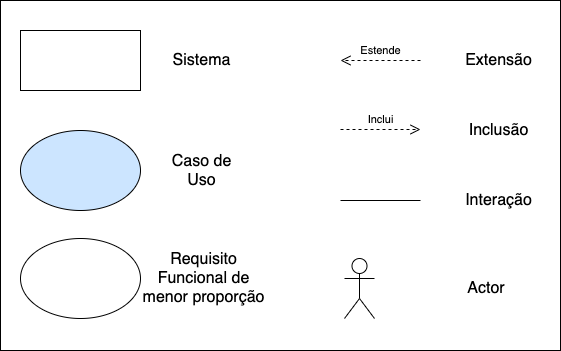
\includegraphics[width=0.7\textwidth]{img/rf/legenda}
		\caption{Legenda dos diagramas}
		\label{fig:rf-legenda}
	\end{center}
\end{figure}


\subsection{Diagrama de contexto}
\label{d:contexto}
\begin{figure}[ht!]
	\begin{center}
		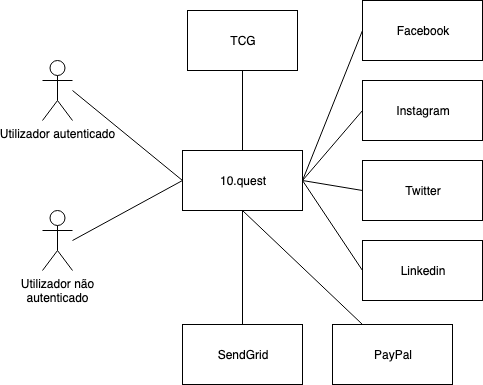
\includegraphics[width=0.6\textwidth]{img/rf/10quest}
		\caption{Diagrama de contexto}
		\label{fig:rf-10quest}
	\end{center}
\end{figure}

\newpage

\subsection{Diagrama de alto nível}
\label{d:altonivel}
\begin{figure}[ht!]
	\begin{center}
		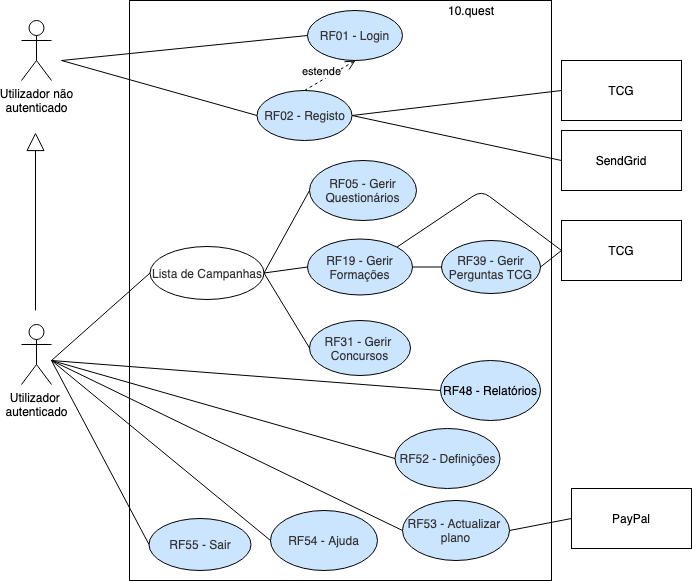
\includegraphics[width=0.8\textwidth]{img/rf/alto-nivel}
		\caption{Diagrama de Alto Nível}
		\label{fig:rf-alto-nivel}
	\end{center}
\end{figure}

\newpage

\subsection{Diagrama Registo}
\label{d:registo}
\begin{figure}[ht!]
	\begin{center}
		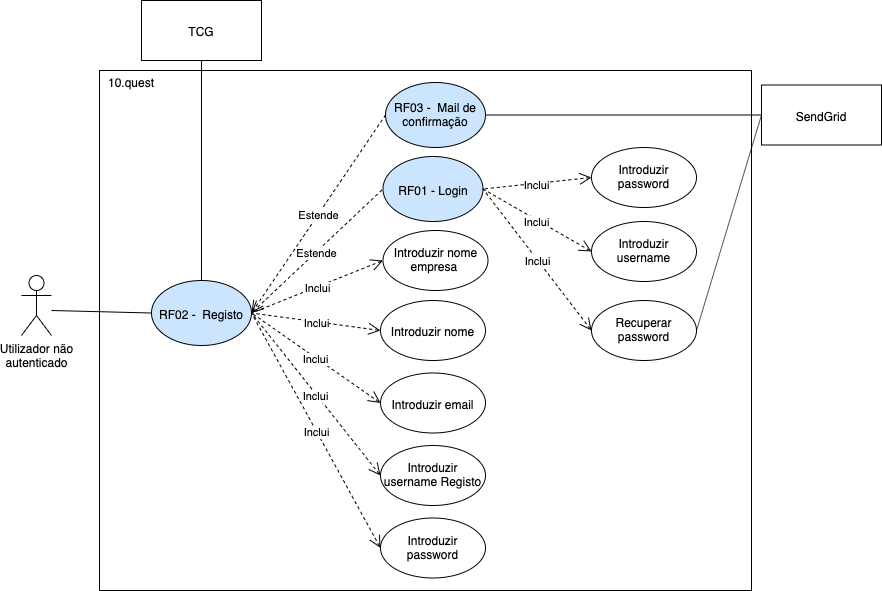
\includegraphics[width=1\textwidth]{img/rf/registo}
		\caption{Diagrama Gerir Concursos}
		\label{fig:rf-registo}
	\end{center}
\end{figure}

\newpage

\subsection{Diagrama Gerir Formações}
\label{d:formacoes}
\begin{figure}[ht!]
	\begin{center}
		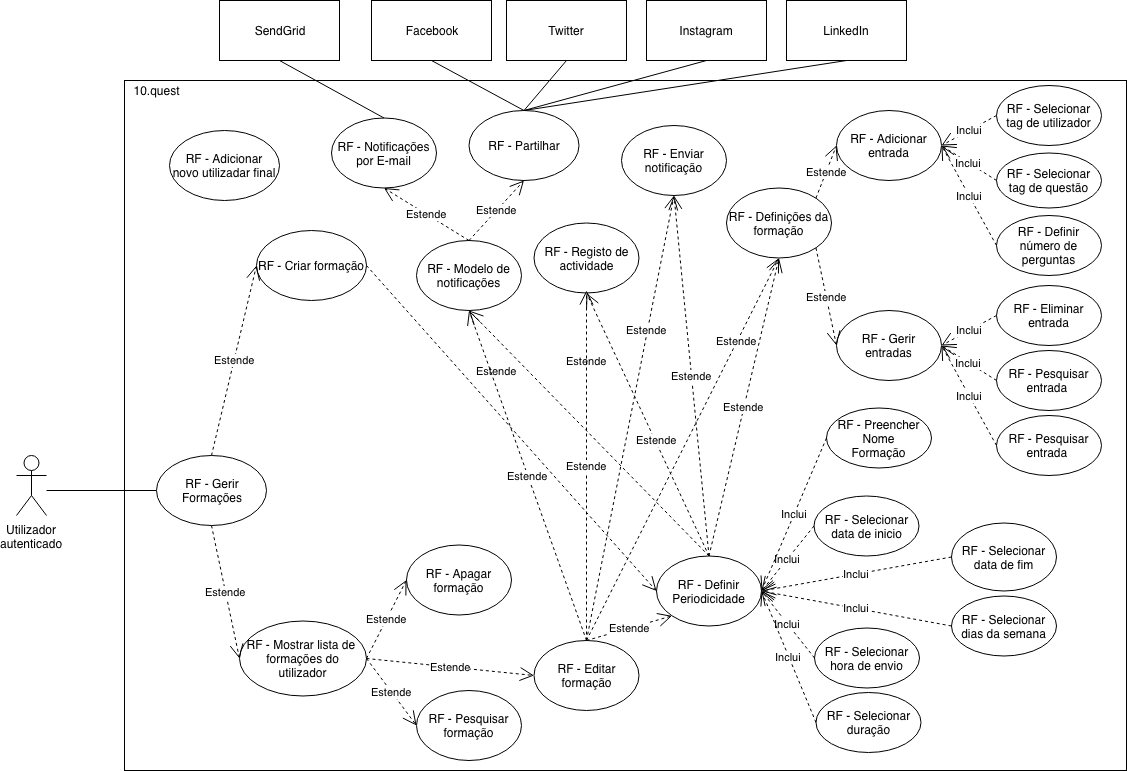
\includegraphics[width=1\textwidth]{img/rf/gerir-formacoes}
		\caption{Diagrama Gerir Formações}
		\label{fig:rf-gerir-formacoes}
	\end{center}
\end{figure}

\newpage

\subsection{Diagrama Gerir Questionários}
\label{d:quests}
\begin{figure}[ht!]
	\begin{center}
		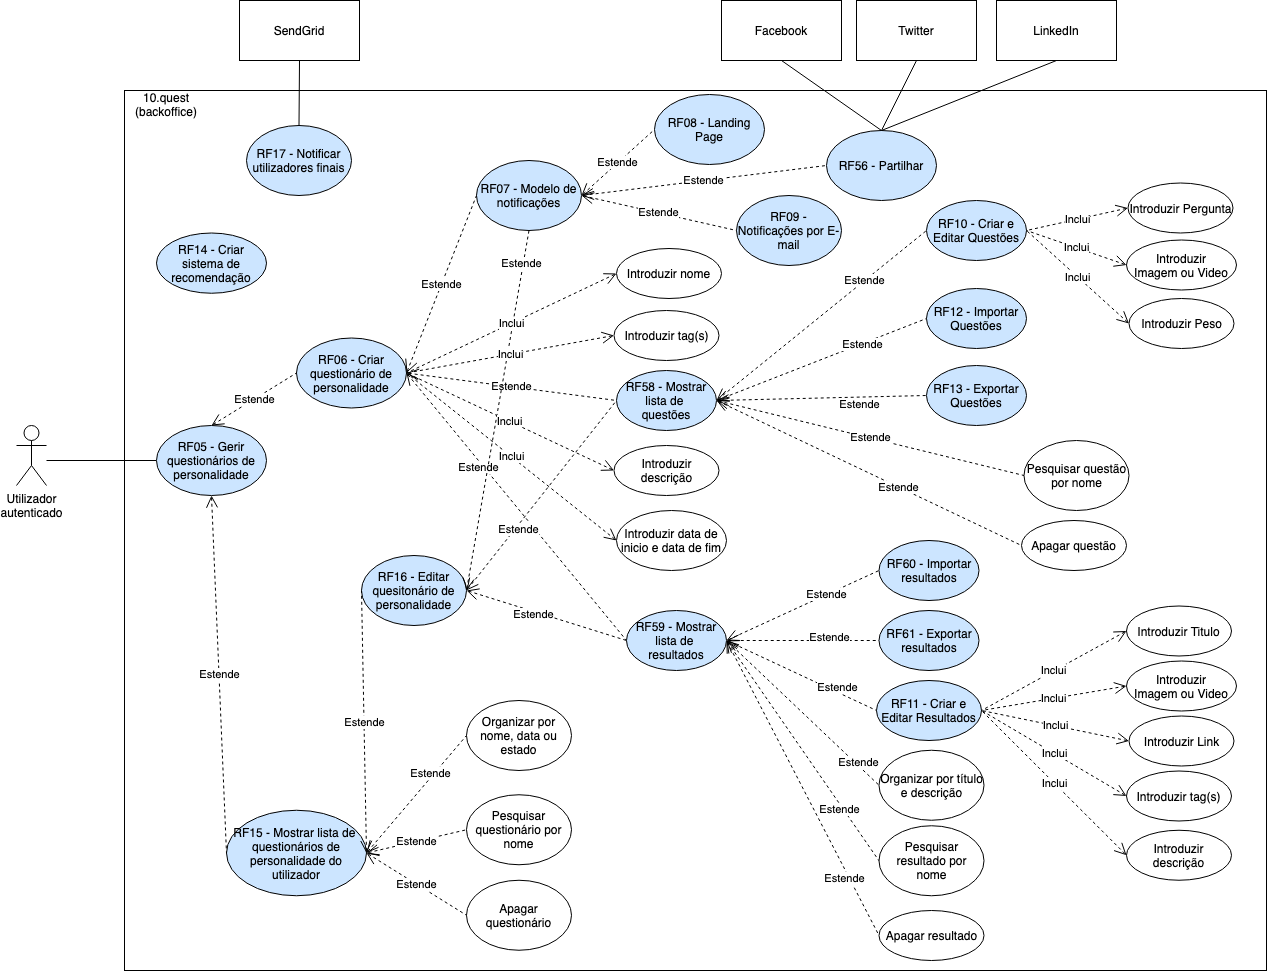
\includegraphics[width=1\textwidth]{img/rf/gerir-quest}
		\caption{Diagrama Gerir Questionários}
		\label{fig:rf-gerir-quest}
	\end{center}
\end{figure}


\newpage

\subsection{Diagrama Gerir Concursos}
\label{d:concursos}
\begin{figure}[ht!]
	\begin{center}
		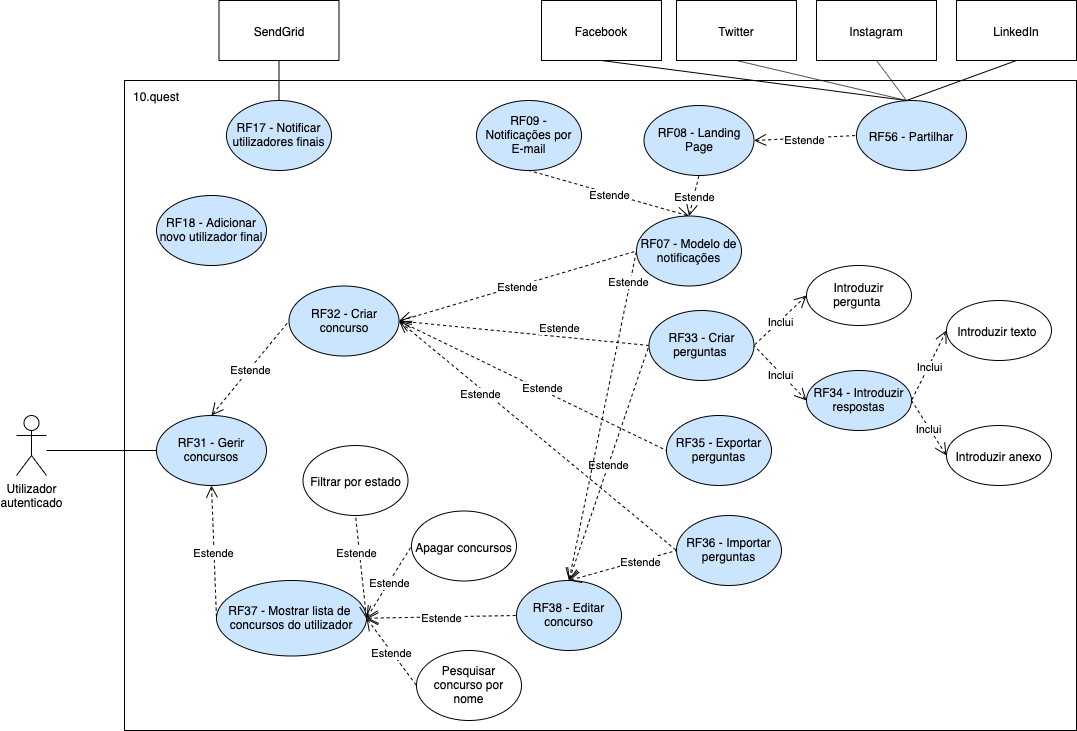
\includegraphics[width=1\textwidth]{img/rf/gerir-concurso}
		\caption{Diagrama Gerir Concursos}
		\label{fig:rf-gerir-concursos}
	\end{center}
\end{figure}


\newpage


\subsection{Diagrama Gerir Perguntas TCG}
\label{d:perguntastcg}
\begin{figure}[ht!]
	\begin{center}
		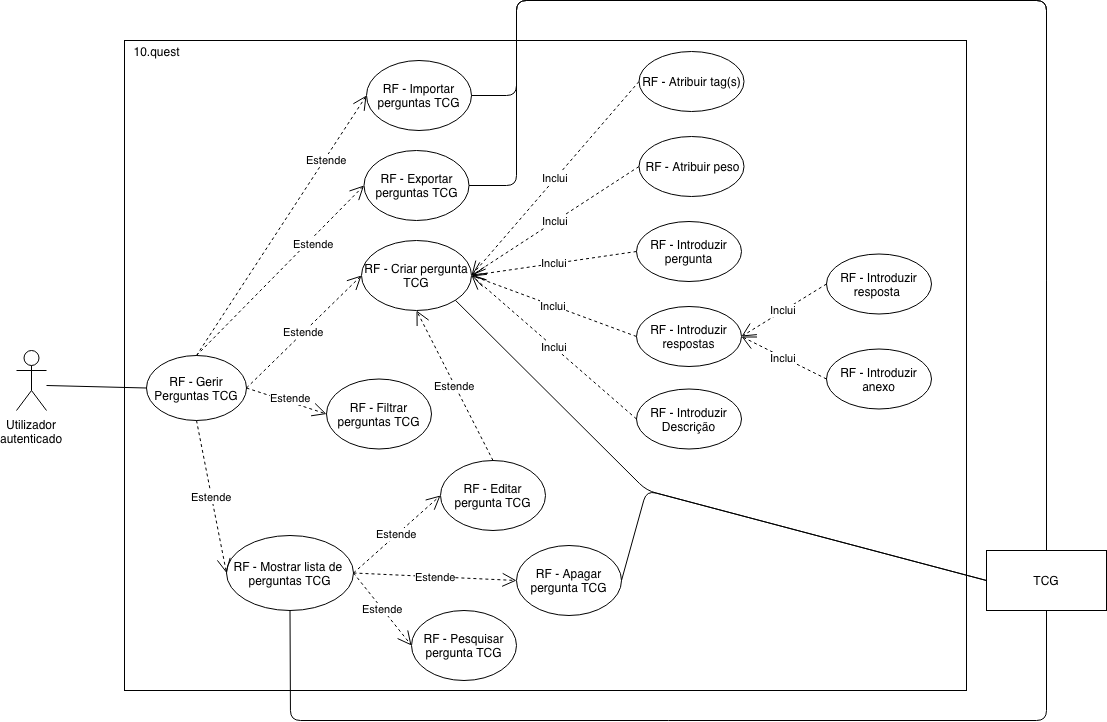
\includegraphics[width=1\textwidth]{img/rf/gerir-perguntas-tcg}
		\caption{Diagrama Gerir Perguntas TCG}
		\label{fig:rf-gerir-perguntas-tcg}
	\end{center}
\end{figure}


\newpage

\subsection{Diagrama Ajuda}
\label{d:ajuda}
\begin{figure}[ht!]
	\begin{center}
		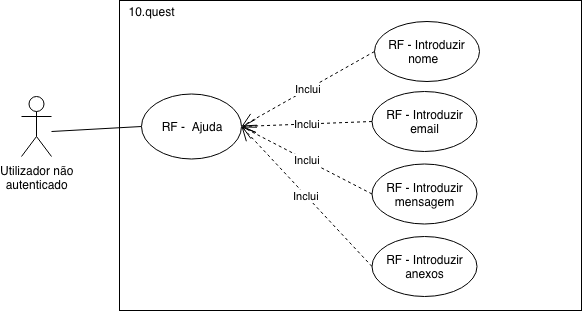
\includegraphics[width=1\textwidth]{img/rf/ajuda}
		\caption{Diagrama Ajuda}
		\label{fig:rf-ajuda}
	\end{center}
\end{figure}




\newpage
\section{Prototipagem}
\label{prototipagem}


%-------------------------------------------------------------------------------------------------
\blankpage
%-------------------------------------------------------------------------------------------------

\glsresetall